\documentclass[11pt, oneside]{article}   	% use "amsart" instead of "article" for AMSLaTeX format
\usepackage{geometry}                		% See geometry.pdf to learn the layout options. There are lots.
\geometry{letterpaper}                   		% ... or a4paper or a5paper or ... 
%\geometry{landscape}                		% Activate for for rotated page geometry
%\usepackage[parfill]{parskip}    		% Activate to begin paragraphs with an empty line rather than an indent
\usepackage{graphicx}				% Use pdf, png, jpg, or eps� with pdflatex; use eps in DVI mode
								% TeX will automatically convert eps --> pdf in pdflatex		
\usepackage{amssymb}
\usepackage{amsmath}
\usepackage{parskip}
\usepackage{color}

\title{Paraboloid}
%\author{The Author}
%\section{}
% \subsection*{R code}
\date{}							% Activate to display a given date or no date

\graphicspath{{/Users/telliott_admin/Dropbox/Tex/png/}}

% \begin{center} 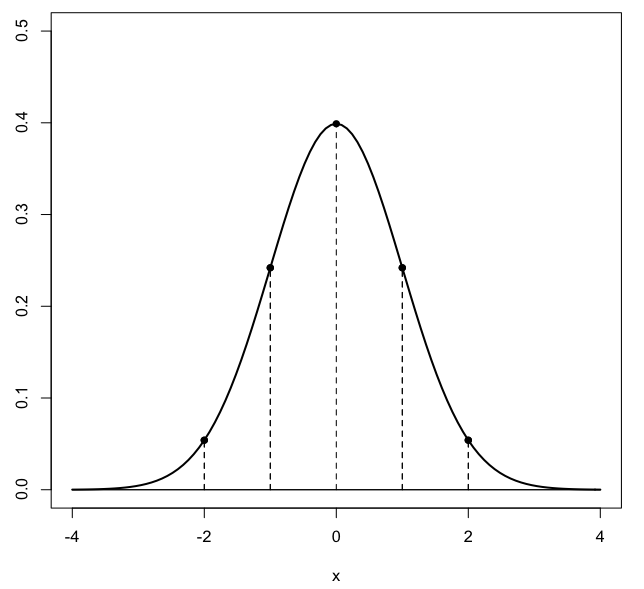
\includegraphics [scale=0.4] {gauss3.png} \end{center}

\begin{document}
\maketitle
\Large
\noindent

Our first example was the paraboloid

\[ z = f(x,y) = 2 - x^2 - y^2 \]

The vertex of this solid is at $(x=0, y=0, z=2)$.  

We can see where the function gets its name.  Visualize the intersection with the $yz$-axis ($x=0$).  There, $z = 2 - y^2$, and we have a standard parabola opening down, with vertex $z=0$.  

The same thing happens at the intersection with the $xz$-axis (where $y=0$ and we have $z = 2 - x^2$).  

Finally, the intersection with the $xy$-axis is $z=0$ so

\[ x^2 + y^2 = 2 \]

 and this is a circle with radius $\sqrt{2}$.

If we view the surface of the paraboloid as enclosing a volume, we can calculate that volume by a double integral of the function over its "shadow" in the $xy$-plane.

\[ V = \iint_R f(x,y) \ dy \ dx \]

We need to figure out the limits on $x$ and $y$.  The outer integral (in $x$) ranges over the whole diameter of the circle from $x = -\sqrt{2} \rightarrow \sqrt{2}$.  For any fixed value of $x$, $y = \sqrt{2 - x^2}$, so the integral can be set up as

\[ \int_{x=-\sqrt{2}}^{x=\sqrt{2}}  \int_{y=-\sqrt{2-x^2}}^{y= \sqrt{2-x^2}}   2 - x^2 - y^2 \ dy \ dx \]
Over the first quadrant
\[ \int_{0}^{\sqrt{2}}  \int_{0}^{\sqrt{2-x^2}}   2 - x^2 - y^2 \ dy \ dx \]


The inner integral is

\[ \int_{0}^{\sqrt{2-x^2}}    2 - x^2 - y^2 \ dy \]
\[ = 2 - x^2 y - \frac{y^3}{3} \ \bigg |_{0}^{\sqrt{2-x^2}} \]
\[ = 2 - x^2 \sqrt{2-x^2} - \frac{(2-x^2)^{3/2}}{3}  \]
\[ = 2 - \sqrt{2-x^2} \ (x^2 + \frac{(2-x^2)}{3})  \]
\[ = 2 - \frac{2}{3} \sqrt{2-x^2} - \frac{2}{3} x^2 \ \sqrt{2-x^2}  \]

And this is going to awkward.  So instead, we go back and use the obvious symmetry and do this in cylindrical coordinates









\end{document}  